%%% Template originaly created by Karol Kozioł (mail@karol-koziol.net) and modified for ShareLaTeX use

\documentclass[a4paper,11pt]{article}

\usepackage[T1]{fontenc}
\usepackage[spanish]{babel}
\usepackage[utf8]{inputenc}
\usepackage{graphicx}
\usepackage{xcolor}
\usepackage{wrapfig}

\renewcommand\familydefault{\sfdefault}
\usepackage{tgheros}
\usepackage[defaultmono]{droidmono}

\usepackage{amsmath,amssymb,amsthm,textcomp}
\usepackage{enumerate}
\usepackage{multicol}
\usepackage{tikz}

\usepackage{geometry}
\geometry{total={210mm,297mm},
left=25mm,right=25mm,%
bindingoffset=0mm, top=20mm,bottom=20mm}


\linespread{1.3}

\newcommand{\linia}{\rule{\linewidth}{0.5pt}}

% custom theorems if needed
\newtheoremstyle{mytheor}
    {1ex}{1ex}{\normalfont}{0pt}{\scshape}{.}{1ex}
    {{\thmname{#1 }}{\thmnumber{#2}}{\thmnote{ (#3)}}}

\theoremstyle{mytheor}
\newtheorem{defi}{Definition}

% my own titles
\makeatletter
\renewcommand{\maketitle}{
\begin{center}
\vspace{2ex}
{\huge \textsc{\@title}}
\vspace{1ex}
\\
\linia\\
\@author \hfill \@date
\vspace{4ex}
\end{center}
}
\makeatother
%%%

% custom footers and headers
\usepackage{fancyhdr}
\pagestyle{fancy}
\lhead{}
\chead{}
\rhead{}
\lfoot{Entrega \textnumero{}  5 - Proyecto Seguridad Informática}
\cfoot{}
\rfoot{Página \thepage}
\renewcommand{\headrulewidth}{0pt}
\renewcommand{\footrulewidth}{0pt}
%

% code listing settings
\usepackage{listings}
\lstset{
    language=Python,
    basicstyle=\footnotesize,
    frame=.2,
  xleftmargin=.2\textwidth, xrightmargin=.2\textwidth,
    basicstyle=\ttfamily\small,
    columns=fixed,
    extendedchars=true,
    breaklines=true,
    tabsize=6,
    prebreak=\raisebox{1ex}[1ex][1ex]{\ensuremath{\hookleftarrow}},
    showspaces=false,
    showstringspaces=false,
    keywordstyle=\color[rgb]{0.627,0.126,0.941},
    commentstyle=\color[rgb]{0.133,0.545,0.133},
    stringstyle=\color[rgb]{01,0,0},
    captionpos=t,
    escapeinside={\%*}{*)}
}

%%%----------%%%----------%%%----------%%%----------%%%

\begin{document}

\begin{titlepage} % Suppresses displaying the page number on the title page and the subsequent page counts as page 1
	
	\raggedleft % Right align the title page
	
	\rule{1pt}{\textheight} % Vertical line
	\hspace{0.05\textwidth} % Whitespace between the vertical line and title page text
	\parbox[b]{0.75\textwidth}{ % Paragraph box for holding the title page text, adjust the width to move the title page left or right on the page
	 \begin{tabularx}{\linewidth}{}
    \makecell{
\includegraphics[height=2cm]{logo}}
     \end{tabularx}
     \bigskip
     \vfill
		{\Huge\bfseries Entrega \textnumero{} 5 Proyecto\\[0.5\baselineskip] Seguridad ~ Informática}\\[2\baselineskip] % Title
		{\large\textsc{Auditoria de la Aplicación y}}\\
		{\large\textsc{Decompilación }}\\[1\baselineskip] % Subtitle or further description
		{\normalsize\textit{Camilo Zepeda Hoffmann}} % Author name, lower case for consistent small caps
		
		\vspace{0.5\textheight} % Whitespace between the title block and the publisher
		
		{\noindent Profesor~ Maximiliano~Vega\plogo}\\[\baselineskip] % Publisher and logo
		{\normalsize\textit{15 de Noviembre 2017}}
	}

\end{titlepage}


\section{Resumen}

Al igual que los incrementales anteriores se dan a conocer los pasos correspondientes a una nueva prueba de auditoría exponiendo las actividades y puntos encontrados a lo largo de la experiencia.



\section{Pruebas y Herramientas}
Se realizan pruebas del tipo interceptoras, con tal de captar información sensible utilizando falseos de certificados y Wireshark. 
Entonces para determinar lograr un mayor comprendimiento de los pasos realizados, se nombra:



\begin{itemize}
    \item \textbf{Paso 1}: se hace uso de la Herramienta Metasploit utilizada para desarrollar y ejecutar exploits contra una máquina remota, generando scripts de utilidad, declarando ejercicios como DoS u otros, de tal manera de generar pruebas dentro de la IP obtenida.
  

    
    \begin{figure}[!h]
    \centering
    
\includegraphics[scale=0.3]{meta.jpg}
    \label{fig:my_label}
    \end{figure}
    
   
    
    
    \item \textbf{Paso 2}: es necesario realizar un ping por CMD de la página atacar, de tal manera de obtener su Ip y datos pertinentes, utilizando el siguiente comando:
    
    \begin{center}
        \textbf{ping www.instagram.com}
    \end{center}
    
    de lo cual se obtiene:
    
    \newpage
     \begin{figure}[!h]
    \centering
    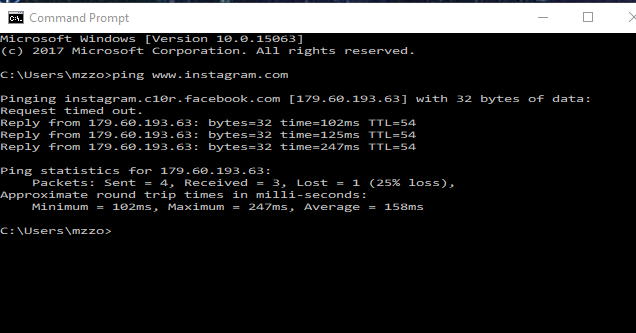
\includegraphics[scale=0.6]{pinginstagram.png}
    \label{fig:my_label}
    \end{figure}
    
    Si bien al realizar el ping se obtiene una ip consistente, tras realizar diversos ping al mismo sitio se generan distintas IP's lo que implica una distribución realizada por parte de los desarrolladores. Aún con la resolución del asunto es posible destacar respuestas por partes del sitio, dando paso a vistas del tipo ICMP. Entonces se logra destacar que existe uso del servidor \textbf{Gunicorn} para manejo de peticiones, el cual a diferencia de Apache es más fácil de implementar y menos intensivo con la CPU, de igual manera para la ejecución de comando se utiliza \textbf{Fabric} como despliegue de ejecución (consultas)
    
    
    \item \textbf{Paso 3}:  Se dispone a utilizar el siguiente comando \textbf{use auxiliary/dos/tcp/synflood}, donde se provee \textbf{auxiliary}, el cual permite la obtención de información sobr el objetivo, con tal de determinar las posibles vulnerabilidades. Además de proveer el protocolo \textbf{tcp} y  el tipo de ataque a realizar, el cual para este caso corresponde a \textbf{dos} y \textbf{synflood} 
      
    
     \begin{figure}[!h]
    \centering
    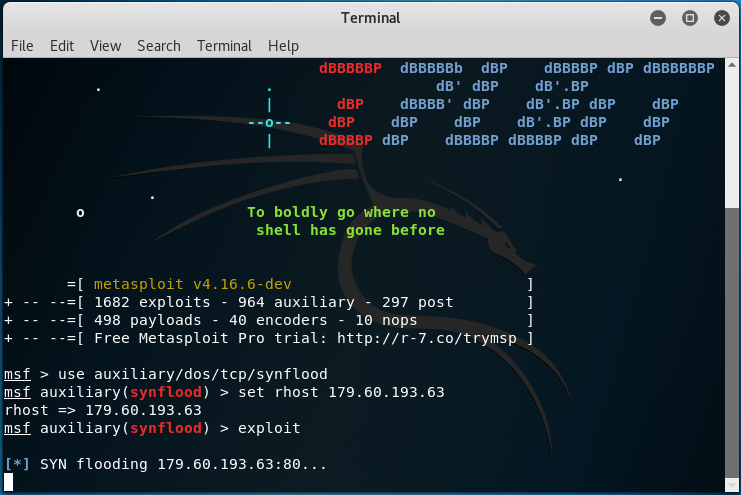
\includegraphics[scale=0.5]{sploit.png}
    \label{fig:my_label}
    \end{figure}
    
 
Entonces tras proveer los comandos necesarios para realizar el ataque es necesario describir el rhost al cual atacar, donde la IP obtenida corresponde al ping generado en el paso anterior, siendo entonces \textbf{179.60.193.63}
 
  \item \textbf{Paso 4}: ya inicializado el ataque se utiliza la herramienta wireshark con tal de ver el envio de paquetes en línea, siendo la respuesta:
  
  \newpage
  
  \begin{figure}[!h]
    \centering
    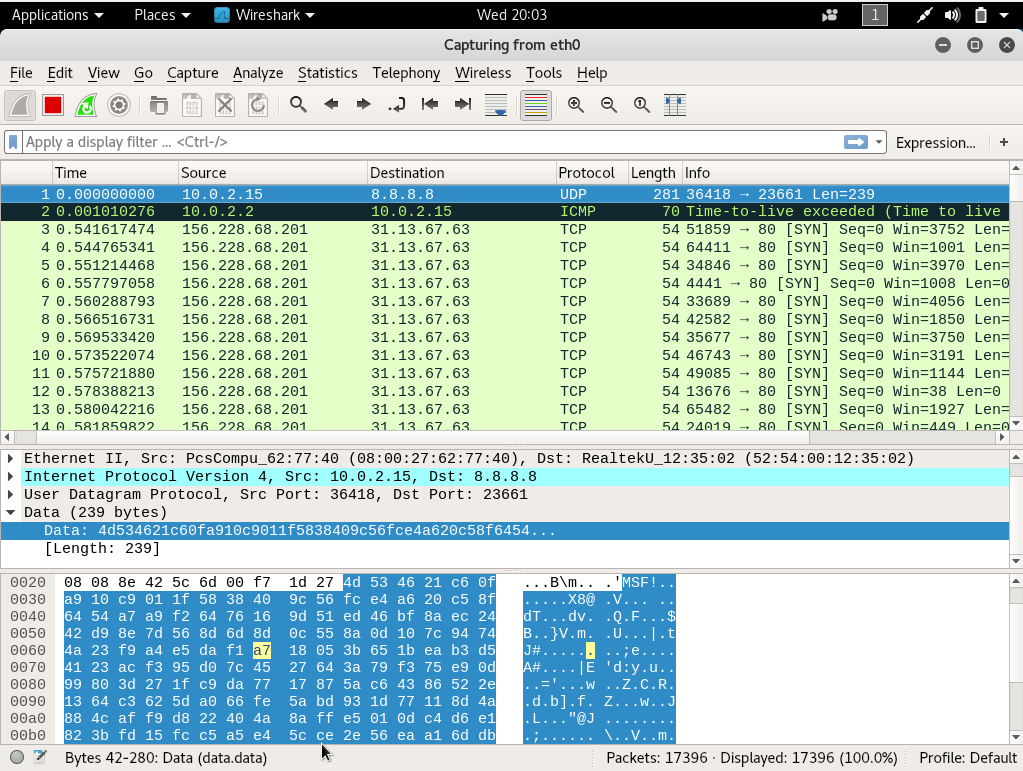
\includegraphics[scale=0.5]{wireshark.png}
    \label{fig:my_label}
  \end{figure}
  
 En la figura anterior es posible apreciar los diferentes paquetes enviados, asociados a sus respectivas respuestas. Cabe destacar, que si bien el ataque se realiza exitosamente no es posible generar un ataque consistente debido a los escasos recursos y lo amplio de la red de la página asociada. 
    
  
\end{itemize}





\newpage










\begin{thebibliography}{1}
\bibitem{Oauth}
www.instagram.com

\bibitem{hack}
http://gunicorn.org/

\bibitem{appirater}
https://www.si6networks.com/presentations/ANTEL07/fgont-antel07-icmp-attacks.pdf

\bibitem{appirater2}
https://github.com/arashpayan/appirater

\bibitem{kali}
https://www.kali.org/

\bibitem{meta}
https://www.metasploit.com/

\end{thebibliography}

\newpage



\end{document}
